% Chapter 2

\chapter{Conceitos} % Main chapter title


%----------------------------------------------------------------------------------------

\section{Inteligência Artificial}

A inteligência artificial (IA) é um ramo cientifico da computação que se dedica ao desenvolvimento de sistemas capazes de executar tarefas que normalmente exigiriam inteligência humana.
Estes sistemas têm a capacidade de executar funções avançadas e analisar dados de grande escala a fim de gerar respostas precisas.  Baseado num conceito do filosofo do grego Aristoteles, a IA surgiu na década de 1950 por Allan Turing, onde o mesmo escreveu sobre a possibilidade de uma máquina pensar e imitar o comportamento humano inteligente. 
Atualmente a IA é aplicada em diversos setores, como na saúde através do diagnostico automatizado de doenças, no setor financeiro para análises de mercado e deteção de fraudes, entre outros. Recentemente a IA sofreu um rápido avanço, com a corrida da IA generativa, sendo o seu componente-chave a fundação da OpenAI em 2015 e surgimento do ChatGPT em 2022, sistema este capaz de processar linguagem natural (NLP) e gerar respostas precisas e corretas sobre variados assuntos (https://hai.stanford.edu/news/ai-spring-four-takeaways-major-releases-foundation-models).

Dentro da IA existem diferentes sub-ramos cientificos, como:

\begin{itemize}
    \item Machine Learning (ML): Ensina computadores a aprender padrões a partir de dados através de redes neronais ou arvores de decisão;
    \item Deep Learning (DL): Sub-ramo do ML que faz uso de redes neronais para modelar a intrepertar padrões complexos;
    \item Processamento de linguagem natural (NLP): Intrepertação de linguagem natural humana.
    \item Visão computacional: Intrepertação de imagens e vídeos
\end{itemize}



\section{Machine Learning \& Deep Learning}

TODO rever secção, AI

O Machine Learning é um subcampo da inteligência artificial centrado no desenvolvimento de algoritmos capazes de identificar padrões em dados e realizar previsões ou decisões com base nesses padrões, sem que para isso sejam explicitamente programados. Esta abordagem baseia-se na experiência — os modelos são treinados com dados históricos e ajustam os seus parâmetros internos para generalizar para novos dados, muitas vezes em contextos altamente variáveis e complexos.

A aprendizagem automática pode ser agrupada em três principais paradigmas:
\begin{itemize}
    \item \textbf{Aprendizagem supervisionada}, em que o modelo é treinado com exemplos rotulados (inputs associados a outputs desejados), aprendendo uma função que generaliza para novos dados;
    \item \textbf{Aprendizagem não supervisionada}, onde o objetivo é descobrir estruturas ou padrões ocultos em dados não rotulados, como agrupamentos ou relações estatísticas;
    \item \textbf{Aprendizagem por reforço}, na qual um agente interage com um ambiente, aprendendo uma política de acções com base num sistema de recompensas, com o objetivo de maximizar um retorno cumulativo.
\end{itemize}

Dentro do ML, destaca-se o Deep Learning, que se baseia no uso de redes neuronais artificiais profundas, compostas por múltiplas camadas de unidades de processamento. Estas redes têm a capacidade de modelar relações não lineares complexas, sendo particularmente eficazes em tarefas como a visão computacional, a tradução automática e o processamento de NLP.

Uma das principais vantagens da aprendizagem profunda reside na sua capacidade de extrair representações hierárquicas dos dados — as camadas iniciais aprendem características de baixo nível, enquanto as camadas superiores capturam abstrações mais elevadas, permitindo uma compreensão mais profunda do domínio em causa. Ao contrário dos métodos tradicionais, que requerem engenharia manual de atributos, o DL automatiza esse processo, o que se revela vantajoso em cenários com grandes volumes de dados.

Estas capacidades fizeram do Deep Learning a base das mais recentes inovações em inteligência artificial, nomeadamente os modelos de linguagem de grande escala 
(Large Language Models – LLMs), que se tornaram uma das áreas mais ativas e transformadoras da IA nos últimos anos.




\section{Large Language Models}

Os LLMs representam um avanço significativo na IA. Proposta pela Google em 2017, atualmente, Transformer é a arquitetura de DL mais explorada para esta componente. Os Transformers foram inicialmente desenvolvidos como melhoria das arquiteturas anteriores para a tradução automática, mas desde então têm encontrado muitas aplicações, como na visão computacional e NLP. Conduziram ao desenvolvimento de sistemas pré-treinados, tais como Generative Pre-trained Transformers (GPTs) and Bidirectional Encoder Representations from Transformers (BERT). Estes modelos são treinados através do paradigma Self-supervised learning (SSL), no qual aprendem representações úteis dos dados sem a necessidade de rótulos manuais. No SSL, o próprio modelo gera os seus rótulos a partir dos dados brutos, criando tarefas preditivas auxiliares chamadas pretext tasks. Masked Language Modeling é um exemplo de tarefa preditiva, utilizada pelo BERT, onde palavras altetórias são ocultadas em uma frase e o modelo aprende a prever as palavras corretas, isto no contexto de NLP. Em contraste o GPT faz uso do Casual Language Modeling onde o modelo prevê a próxima palavra numa sequência de texto, dado o contexto anterior.

TODO melhorar texto abaixo 

O aumento da escala destes modelos — tanto em volume de dados como em parâmetros — contribuiu para ganhos significativos em capacidades linguísticas, raciocínio e compreensão contextual. Os LLMs modernos, como os da família GPT, constituem atualmente a espinha dorsal de sistemas conversacionais, motores de busca inteligentes, e aplicações empresariais que requerem compreensão profunda da linguagem.

\section{Fine-tuning LLMs}

 TODO e depois no RAG fazer uma comparação e mostrar vantagens do RAG

\section{Retrieval-Augmented Generation}

Apesar dos avanços dos LLMs, estes modelos enfrentam limitações em ambientes onde o acesso a conhecimento atualizado ao contexto é crucial. A técnica de fine-tuning abordada anteriormente é dispendiosa e não escala bem para conteúdos em constante mudança. Retrieval-Augmented Generation (RAG) surge como uma solução alternativa, permitindo enriquecer a geração com acesso em tempo real a fontes externas.

RAG é uma técnica que combina LLMs com um mecanismo de recuperação de informação externa. Enquanto que os LLMs apenas se baseiam em dados pré-treinados, o RAG recupera informação relevante de um contexto específico armazenado previamente.

Tendo em consideração que RAG é a peça fundamental de estudo do presente documento, nesta secção serão abordados todos os seus conceitos mais importantes.

\subsection{Arquitetura}


O fluxo típico do RAG encontra-se descrito na Figura \ref{fig:acrh-rag}. O processo concentram-se em primeira instancia na formulação da questão (\textit{query}) a ser requisitada ao sistema. De seguida o Retrieval, Augmentation e Generation ocorrem de forma sequencial: 


\begin{itemize}
    \item \textbf{Retrieval}: Baseado na \textit{query}, a função do \textit{Retriever} é percorrer o conhecimento disponível e encontrar informação que vá de encontro a essa \textit{query}. Funciona como uma espécie de motor de busca e é essencial pois determina a relavância e qualidade da informação que será usada para gerar a resposta final. O métodos de recuperação serão discutidos na secção \ref{recu-context}.
    \item \textbf{Augmentation}: O processo de \textit{augmentation} TODO acabar raciocínio
    \item \textbf{Generation}: O \textit{Generator} atua após o \textit{Retriever} ter feito a recuperação de informação relevante, juntando-a com a \textit{query} original para elaborar uma resposta contextualizada. O conhecimento pré-existente é tido em conta pelo o LLM permitindo que as respostas sejam mais inteligentes e informadas para o contexto em questão. 
\end{itemize}


https://medium.com/@sandyeep70/understanding-rag-evolution-components-implementation-and-applications-ecf72b778d15



\begin{figure}[H]
        \centering
        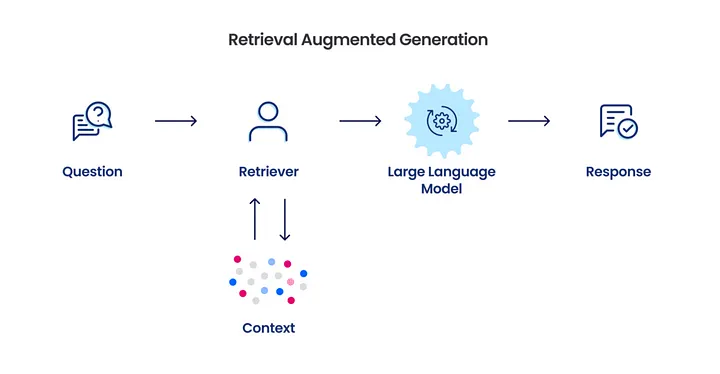
\includegraphics[width=0.7\linewidth]{ch2/assets/RAG-ach.png
        }
        \caption{Arquitetura simplificada do RAG - https://medium.com/@sahin.samia/what-is-retrieval-augmented-generation-rag-in-llm-and-how-it-works-a8c79e35a172}
        \label{fig:acrh-rag}
\end{figure}


\subsection{Persistência do Contexto}

TODO indexação e formas de guardar o contexto

\subsubsection{Bases de Dados Vetoriais}

TODO

Conceito de embeddings e busca vetorial.
Exemplos de ferramentas (FAISS, Weaviate, Pinecone).<
Importância da base vetorial no contexto do RAG.


\subsection{Recuperação do Contexto}
\label{recu-context}

TODO modelos retriever
TODO tipo isto https://docs.llamaindex.ai/en/stable/examples/retrievers/bm25_retriever/


\subsection{Geração do Input LLM}

TODO

\subsection{Prompt Engineering}

TODO

\subsection{Aplicações Práticas}

TODO 

RAG é atualmente usado, por exemplo, para suporte ao consumidor através da criação de Chatbots capazes de recuperar FAQs e o conhecimento do negócio de forma fácil. Gestão do conhecimento empresarial é outro exemplo de caso de uso, pois permite que os funcionários recuperarem e acedam a informação do contexto de trabalho de forma mais rápida. Este último caso de uso vai de encontro aos objetivos do presente projeto. 



\section{Aplicação ao Suporte Técnico}

Como esses conceitos são aplicáveis ao problema da dissertação.
Benefícios esperados da implementação.
